\section{Dynamic and Geometric Analysis of ResNet-LDDMM, and How it Builds Diffeomorphisms}
\label{sec:Diffeos}

\subsection{Regularity of the Deformations}
Each building block $f(\cdot,\theta^l)$ of ResNet-LDDMM can be seen as a vector field on $\real^3$, that is, a mapping $\real^3\rightarrow\real^3$. This yields the transformations $\Phi^l:\real^3\rightarrow\real^3$
\begin{equation} \label{Eq:discreteDiffeo}
\begin{split}
&\forall x\in\real^3,\ l\in \{1,\dots,L\},\\ &\Phi^0(x)=x, \\&\Phi^l(x)=\Phi^{l-1}(x)+ f(\Phi^{l-1}(x),\theta^l).\Delta^L.
\end{split}
\end{equation}
Then, applying $\Phi^l$ separately to each point of the source shape $q_0$, we get the deformed shapes $q^l=\Phi^l.q_0$. Moreover, for a given $x\in q_0$, each $f^l$ is actually computed explicitly (using Eq. (\ref{Eq:vectorFields})) by,
\begin{equation} \label{Eq:vectorFields}
f(x,\theta^l) = w_3^l(w_2^l((w_1^l x+b_1^l)^++b_2^l)),
\end{equation}
with $w_i^l$ matrices whose entries are made up of the parameters $\theta^l$, along with the real numbers $b_j^l$, and $r^+=\max(r,0)=ReLU(r)$, for every real number $r$, is the ReLU function. Each $f(\cdot,\theta^l)$ is Lipshitz, with Lipshitz constant at most equal to the product of the matrix norms of $w_1^l,w_2^l$ and $w_3^l$. The fact that the corresponding transformation is a diffeomorphism can mostly be deduced from  \cite{rousseau2020residual}, but because of minor differences, we give a quick summary of a proof in the following (with details in the Appendix). The system (\ref{Eq:discreteDiffeo}) is a forward Euler algorithm for the flow of the ODE $\partial_t\phi(t,x)=f(x,\theta(t))$, for $x$ in $\real^3$, $t$ in $[0,1]$, and $\theta(t)=\theta^l$ on the interval $[(l-1)\Delta L,l\Delta L)$. Hence, $\phi$ is the flow of the time-dependent vector field $f$, whose Lipshitz constant in space is always less than the maximum $\mathcal{M}$ over $l$ of the product of the matrix norms of $w_1^l,w_2^l$ and $w_3^l$. Therefore, $\phi(t):\real^3\rightarrow\real^3$ exists for all time $t$ in [0,1], and is a bilipshitz map for all $t$. Grownall's lemma also ensures that its Lipshitz constant and that of its inverse is less than $e^{t\mathcal{M}}$. As a final note, should smoothness be required, the ReLu can be replaced by a smooth approximation $g$ with bounded derivative. In this case, the velocity fields will be as smooth as $g$ and the transformation $\Phi$ will then truly be a diffeomorphism. However, as shown in our various experiments, this does not appear necessary, and doing so intrinsically causes the loss of one of the strong points of our approach compared to classical LDDMM: the absence of a scale (see Sec. \ref{sec:LDDMMcomparison}).

\subsection{Geometric Description of the Velocity Fields and Interpretation}
\label{sec:GeometricDescription}

For fixed $l$, the vector fields $f^l(\cdot,\theta^l)$ given by the $l$-th building block have a nice geometric interpretation, which helps understand the way ResNet-LDDMM functions work and the areas in which it improves upon some of the classical LDDMM's weaknesses. For readability, we will omit the index $l$ for now. Recall that $m$ denotes the width of the network. For a fixed parameter $\theta$ of a building block $f(\cdot,\theta)$ of our network  (i.e., a velocity field $x\mapsto f(x,\theta) $), the first layer is the affine transformation $L_1:x\in\real^3\mapsto w_1x+b_1\in \real^m$, with $w_1$ being an $m\times 3$ matrix and $b_1=(b_{1,1},\dots,b_{1,m})$ in $\real^m$. Let us now note $n_1,\dots, n_m\in \real^3$ the vectors whose transposes are the lines of $w_1$; that is, $w_1=(n_1,\dots,n_m)^T$. Then $L_1(x)^T=(n_1^Tx+b_{1,1},\dots,n_m^Tx+b_{1,m})$. 

The second layer $L_2:\real^m\rightarrow\real^m$ is a ReLU function, so that
\begin{equation}\begin{split}
    L_2\circ L_1(x)^T=&((L_2\circ L_{1})_1(x),\dots,(L_{2}\circ L_1)_m(x))
    \\=&((n_1^Tx+b_{1,1})^+,\dots,(n_m^Tx+b_{1,m})^+)
    \end{split}
\end{equation}

Geometrically, a vector $n\in \real^3$ and a number $b\in \real$ define an affine plane $P$ of $\real^3$ through the equation $n^Tx+b=0,\ x\in\real^3$. This separates $\real^3$ into two half spaces: $E^+=\{x\in\real^3, \ n^Tx+b\geq 0\}$ on the side of $P$ towards which $n$ is pointing, and $E^-=\{x\in\real^3, \ n^Tx+b<0\}$, on the other side of $P$. Then, for any $x$ in $\real^3$, we have that the function

\begin{equation}\begin{split}
    D_{n,b}(x)=&(n^Tx+b)^+\\
    =&\left\lbrace\begin{split}n^Tx+b\ \text{if}\ x\in E^+,\\
    0 \text{ if}\ x\in E^-.\end{split}\right.
    \end{split}
\end{equation}
%On $E^+,\ n^Tx+b=\Vert n\Vert_2d(x,P)$, with $d$ the Euclidean distance, so $D_{n,b}$ is actually just proportional to the distance to $P$ in that half-space. 
Then we notice that for $k=1,\dots, m$, the k-th component of $L_2\circ L_1$ is just $(L_2\circ L_1)_k=D_{n_k,b_k}$. 

Hence, the choice of parameters for the first two layers is equivalent to choosing $m$ oriented affine planes $P_1,\dots,P_m$ with corresponding Cartesian equations $n_k^Tx+b_k=0$, $k=1,\dots,m$, and half-spaces $E_k^{\pm}$, obtaining the corresponding components $D_k=D_{n_k,b_k}$. %Geometrically, for $k=1,\dots,m$, each $n_k$ and $b_k$ defines in $\R^3$ an affine plane $P_k$, with normal vector $n_k$ and equation $n_k^Tx+b_k=0$. This separates $\R^3$ into two half-spaces: $E_k^+=\{x\in\real^3, \ n_k^Tx+b_k\geq 0\}$ on the side of $P_k$ towards which $n_k$ is pointing, on which $(L_2\circ L_1)_k(x)=n_k^Tx+b_k$ and $E_k^-=\{x\in\real^3, \ n_k^Tx+b_k\leq 0\}$ on which $(L_2\circ L_1)_k(x)=0$. Note that on $E_k^+,\ n_k^Tx+b_k=\Vert n_k\Vert_2d(x,P_k)$, so $(L_2\circ L_1)_k(x)$ is (essentially) just proportional to the distance from $x$ to $P_k$ in that half-space.
The third and fourth layers of the building block simply combine into an affine transformation $\real^m\rightarrow \real^3$. Therefore, each of the three components of the entire building block $f(.,\theta):\real^3\rightarrow\real^3$ is just an affine combination of the functions $D_k$. In other words, for some vectors $a_1,\dots,a_m$ and $c$ in $\real^3$, we have
\begin{equation}\label{eq:GeometricVelocityFields}
    f(x,\theta)=a_1D_1(x)+\dots+a_mD_m(x)+c.
\end{equation}

Now, take a finite sequence of symbols $\epsilon = (\epsilon_1,\dots,\epsilon_m)$ with each $\epsilon_k$ being either $+$ or $-$, and consider the subset $\displaystyle T_\epsilon=\cap_{k=1,\dots,m} E_k^{\epsilon_k}.$ The domain $T_\epsilon$ is a polytope, that is, a possibly unbounded polyhedron. Then, for every $k$ such that $\epsilon_k=-$, $D_k(x)=0$, and for every other $k$, $D_k(x)=n_k^Tx+b_k$. Plugging this formula into Eq.(\ref{eq:GeometricVelocityFields}), we get
\begin{equation}\label{eq:GeometricVelocityFieldsT}
\begin{split}
    f(x,\theta)=&\sum_{k,\epsilon_k=+}(\underset{\text{3 by 3 matrices}}{\underbrace{a_{kn_k^T}}x}+b_k)+c
    \\
    =&\left(\sum_{k,\epsilon_k=+}a_{kn_k^T}\right)x+\sum_{k,\epsilon_k=+}b_k+c
    \\
    =&A_{\epsilon}x+c_\epsilon.
\end{split}
\end{equation}
In other words, on each $T_\epsilon$, $f(\cdot,\theta)$ is just an affine vector field. In conclusion, each building block of our network, that is, each velocity field we use to construct our final transformation, is just a globally continuous (even globally lipshitz), piece-wise affine mapping, defined on a partition by $2^m$ disjoint polytopes of $\R^3$. 

The optimization of the final network, ResNet-LDDMM, can therefore be thought of as searching for:
\begin{enumerate}
    \item The optimal partition of $\real^3$ into polytopes by $m$ planes at each step
    \item The correct affine transformation on each of these polytopes.
\end{enumerate}
While there are obviously some additional constraints (for example, the transformations need to be globally continuous), this description gives a good representation of what ResNet-LDDMM does. As a result, different parts of the shape, even if they are close in $\real^3$ (such as two fingers on a hand) can be made to belong to different polytopes, and therefore be moved in different directions without costing too much energy (see Fig. \ref{Fig:Directions}). 

\begin{figure} [ht!]
  \centering
  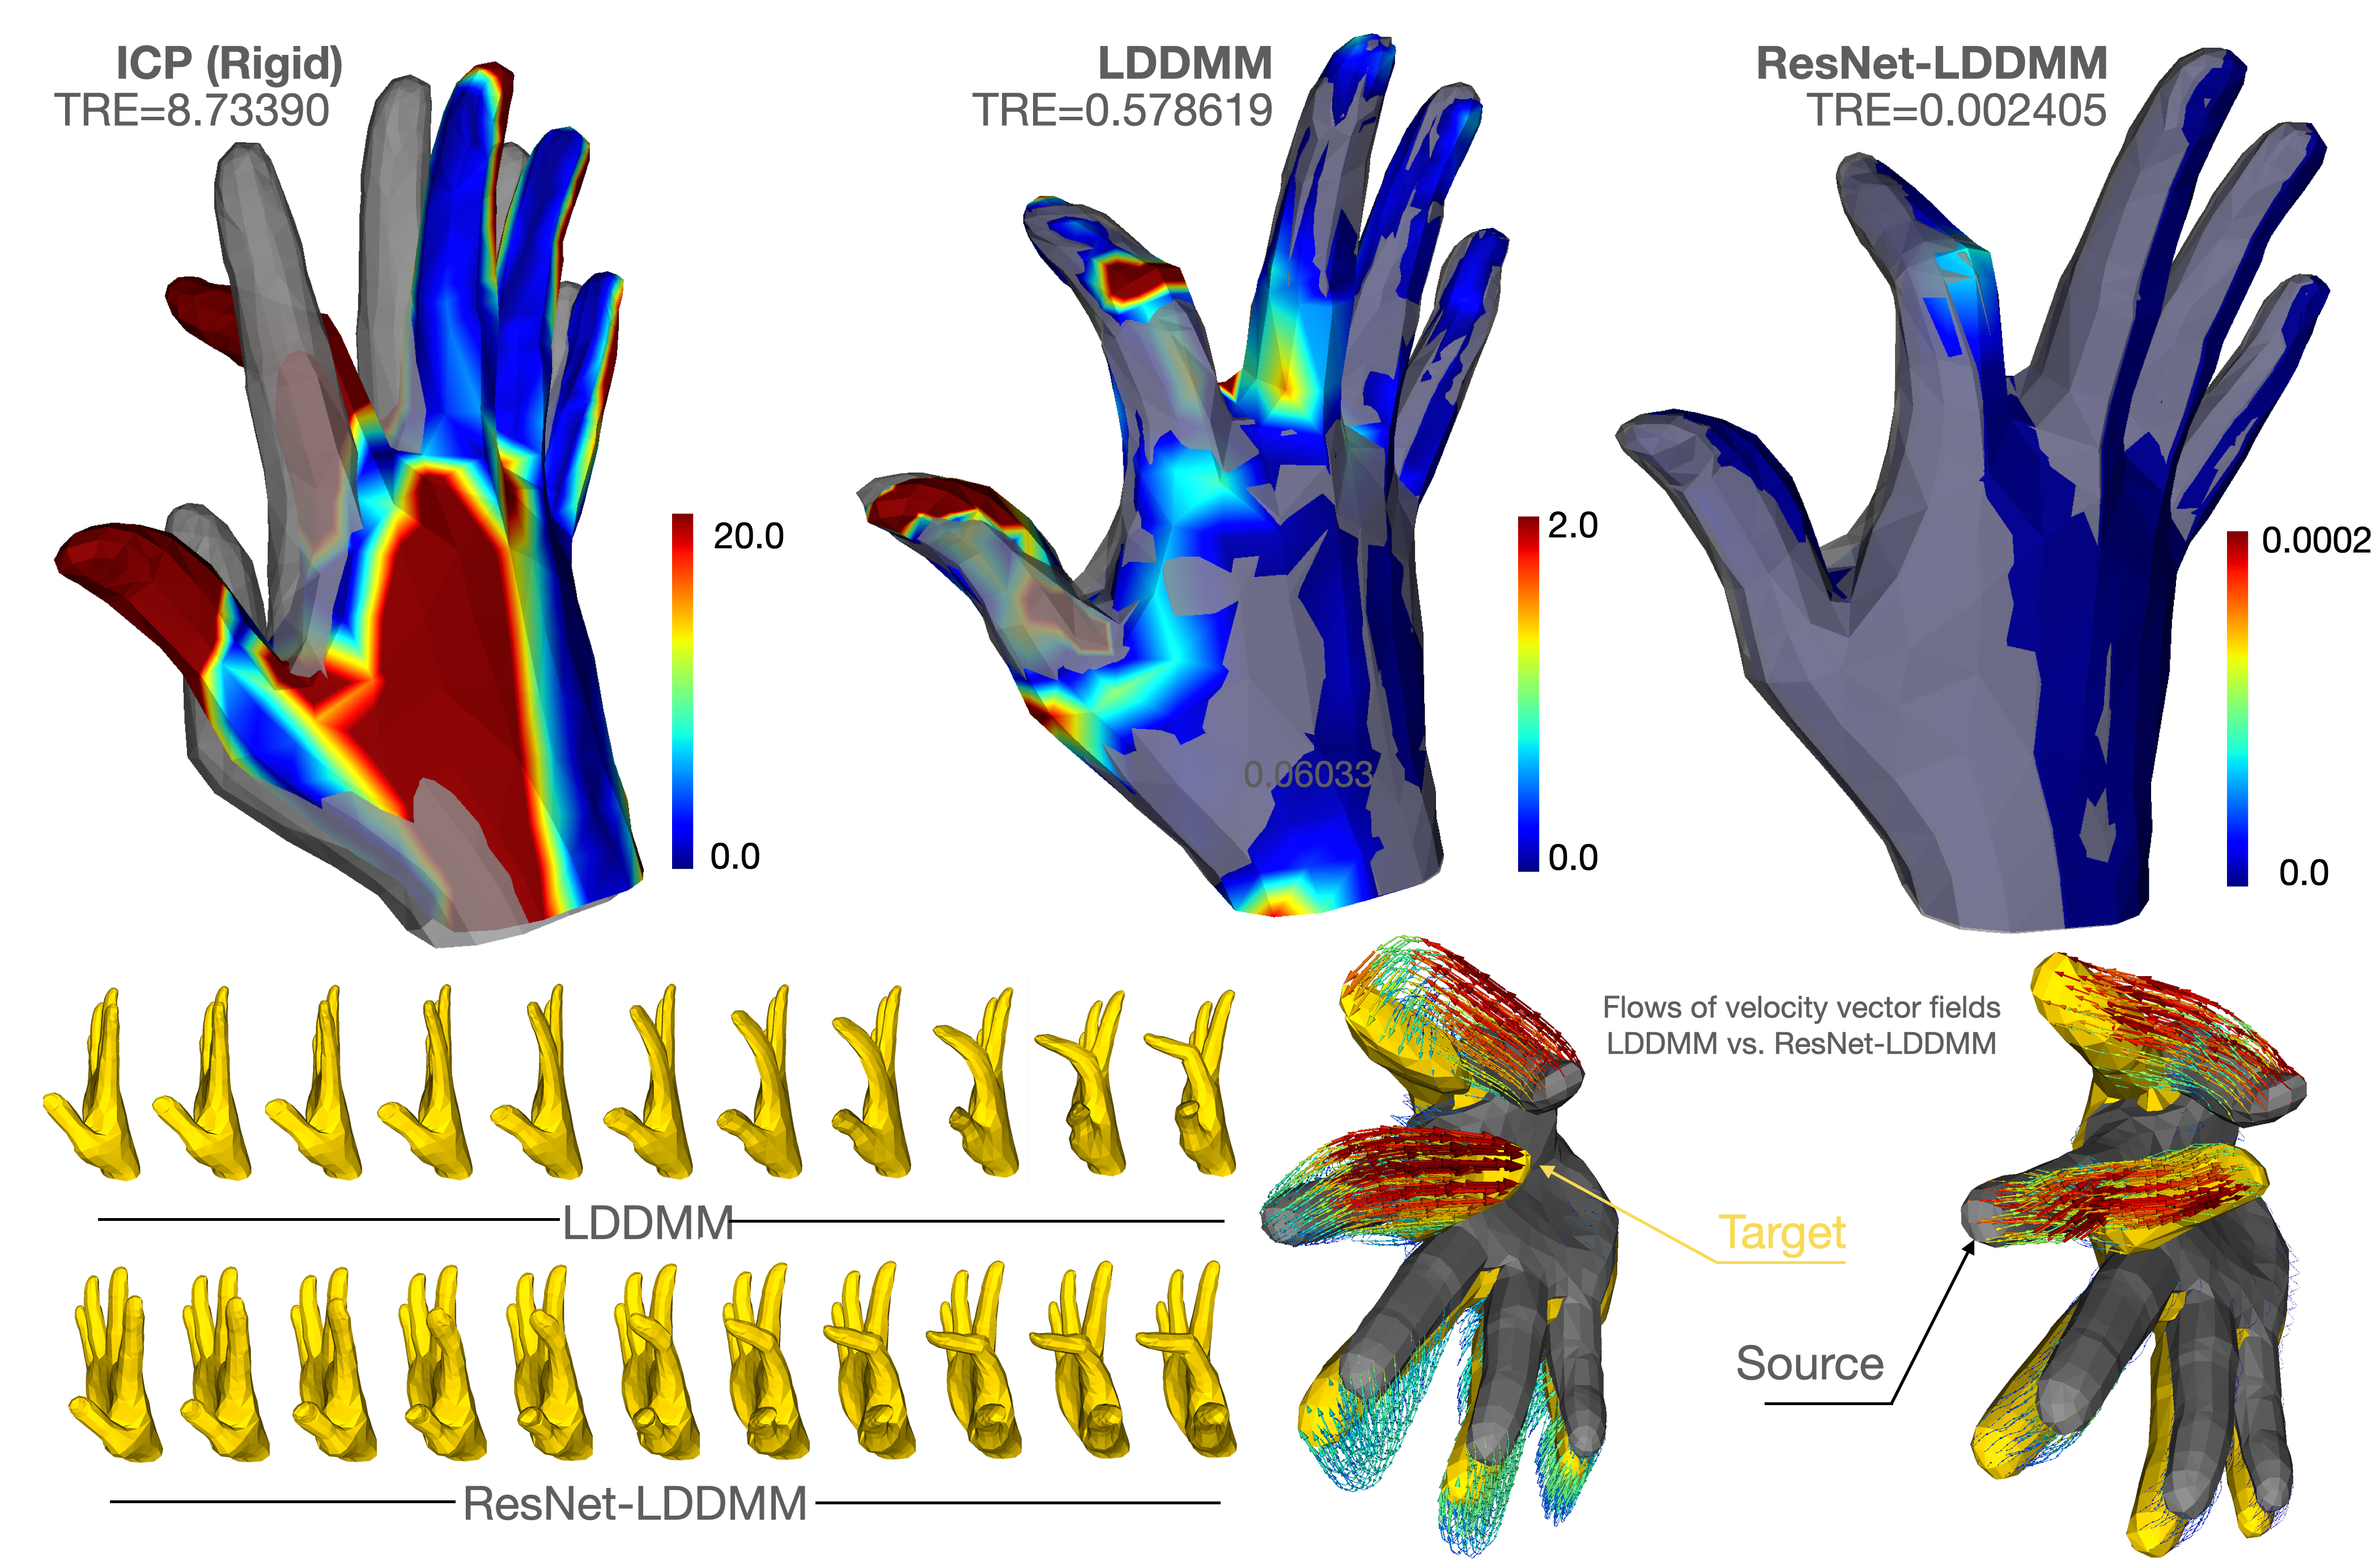
\includegraphics[width=\linewidth]{Figs/Directions2.png}
%   \vspace{-0.8cm}
  \caption{LDDMM vs. ResNet-LDDMM -- registration results of hand shapes with fingers moving in opposite directions.}
   \label{Fig:Directions}
\end{figure}

%\textcolor{red}{Let us give a quick interpretation and explanation for the use of our particular regularization term.}

\subsection{Regularization Term}
\label{sec:GeometricRegularization}

Let us first give a reason not to use (or at least not to only use) a more classical regularization term on the parameters $\theta^l$. Keeping in mind the dynamical interpretation of ResNet-LDDMM, such a term would be given by $\frac{1}{L}\sum_{l=1}^L\Vert\theta^l\Vert^2_{2}$, possibly multiplied by a weight, and corresponds to $\int_0^1\Vert\theta(t)\Vert^2_{2}$dt in the continuous model. However, since each residual layer $f(\cdot,\theta^l)$ is, piecewise, a polynomial of degree three with in the parameters of $\theta^l$, a regularization on $\theta^l$ does not give a good control on its Lipschitz constant. In the network itself, that is not too much of a problem, since boundedness is still ensured. However, in the continuous model, it would be possible to have parameters $\theta(t)$ that have bounded $L^2$ norm, but induce velocity $f(\cdot,\theta(t))$ whose Lipshitz constant $k(t)$ is not integrable. This would prevent it from integrating  into a well-defined diffeomorphism. Indeed, just take each coordinate of $\theta(t)$ to be $\frac{1}{t^{1/3}}$. Then $\Vert\theta(t)\Vert^2_{2}\simeq \frac{1}{t^{2/3}}$ is integrable, but the Lipshitz constant $k(t)\simeq\theta(t)^3\simeq\frac{1}{t}$ is not. This is a known problem in optimal control and shape analysis, and almost always prevents the existence of a global minimizer. See \cite{mumford2006riemannian} for example.

Instead of a regularization term on the parameters $\theta^l$, we use the sum of the kinetic energies of the paths taken by each point of the shape along the deformation \eqref{Eq:ResNet-LDDMM}, which is equal to
$$
\frac{1}{2}\sum_{i=1}^n\int_0^1\Vert f(\Phi(x_i,t),\theta^t)\Vert_{\ell^2}^2dt.
$$
If we had enough degrees on freedom on $\theta$, the optimal deformation $\Phi^*$ with parameters $\Theta^*$ would then be such that every  curve $t\in[0,1]\mapsto \Phi(x_i,t)$ is a straight segment of constant speed, since those minimize the kinetic energy, making the whole algorithm rather pointless. In LDDMM, this happens when the scale becomes much too small. For ResNet-LDDMM, it would correspond to a network width that is too large, allowing each point to belong to a single polytope  with complete control on the affine transformation inside this polytope (as described in the previous section, Section \ref{sec:GeometricDescription}). However, for smaller width, at each residual layer $l$, each polytope $T$ will contain several points of the shape. Then, as long as four those points are not co-planar, the affine mapping $A$ induced by $f(\cdot,\theta^l)$ on $T$ is completely described by its value at those points. As a result, the lipshitz norm of $A$ is indeed controlled by the Euclidean norm of the values of $A$ at those points.





%\textcolor{red}{In addition to all these theoretical explanations, in our experiments, a kinetic only regularization worked much better than a parameter regularization. Using both simultaneously did not seem to improve upon just a kinetic term.} 
%\subsection{Connection with Kernel Methods}\label{sec:NTK}

%The recent theoretical studies on the relationship between Deep Neural Networks and kernel methods in machine learning (e.g. \cite{bietti2019kernel}) make possible to better understand how ResNet-LDDMM works. In fact, each building block $f^l$ (we will omit $l$ later) of ResNet-LDDMM is associated to velocity field and thus allow to predict intermediate coordinates (in $\real^3$) of any $x \in q_S$ till a final state close to $q_T$. Roughly speaking, while ResNet-LDDMM makes such a prediction in an \textbf{unsupervised} way, a supervision is introduced on the source point cloud accounting for 3D points positions in the space. That is, once the ResNet-LDDMM optimized (or trained) and optimal parameters found, the model could be used to predict for any previously unseen point (could be an additional landmark on $q_0$) its new position in the deformed source, $q^L=\Phi^L.q_0$. So that, the all the points in the source shape served, through their coordinates, to train the models $\{f^1,\dots,f^L\}$ while controlling the kinetic energy of the system.  

%In particular, it has been demonstrated in \cite{jacot2018neural,arora2019exact,lee2018deep} that at the infinity width-limit of $f^l$, a.k.a. $w \to \infty$, these functions are equivalent to samples drawn from a \textit{Gaussian} process. When trained by gradient descent with infinitesimal learning rate  (a.k.a. gradient flow) $f^l$ is equivalent to a (linear) kernel regression predictor with a deterministic kernel called Neural Tangent Kernel (NTK) given by Eq.(\ref{Eq:NTK}),

%\begin{equation}
%\mathrm{ker} \left(x,x’\right) = \mathbb{E}_{\theta \sim \Theta}\left[\left\langle \nabla_{\theta} f(x,\theta), \nabla_{\theta} f(x',\theta)\right\rangle\right], 
%    \label{Eq:NTK}
%\end{equation}

%$\quad \forall x, x' \in q_0$. That is, the NTK is defined through the inner product between the gradients of $f$ with respect to the network parameters $\theta$. This in some how reveals an intersection between ResNet-LDDMM, which under a wide-width assumption make use of an RKHS induced by the NTK kernel, and LDDMM which use an RKHS induced by a Gaussian Kernel with a predefined scale. For both cases, The RKHS norm $\|.\|_{\cal H}$ acts as a natural regularization function, which controls the variations of model predictions according to the geometry induced by the NTK. That is, if the feature map which give rise to the induced NTK given by $\phi(x)=\nabla_{\theta} f(x,\theta^0)$, then the variations of a $f$ is controlled according the the geometry induced by the NTK Kernel. We can write Eq.(\ref{Eq:NTKGeom}),

%\begin{equation}
%| f(x) - f(x')| \leq \|f\|_{\cal H}.\|\phi(x) - \phi(x')\|_{\cal H}
%\label{Eq:NTKGeom}
%\end{equation}

%This shows clearly that our fully-connected networks $f$ (each time-step of ResNet-LDDMM) brings a natural regularization through the Hilbert norm of the feature map $\phi$. Accordingly, neighboring points in $x,y \in q^l$ will move similarly, to some extend (related to the constant $\|f^l\|_{\cal H}$ of Eq.(\ref{Eq:NTKGeom})), according to quite similar velocity vectors $f_x^l, f_y^l \in {\cal H}$. This puts additional insights how regular are generated vector fields at time-steps of ResNet-LDDMM, as can be appreciated in Fig.\ref{Fig:VelocityFields}. While we carefully make this interpretation, as our $f$ aren't infinite width, we report in our ablative study (Sec.\ref{sec:ablative}) relevant experiments which study the width's effects on the registration as well as the role of the \textit{kinetic} regularizer in ResNet-LDDMM.  

%\subsection{Key differences with LDDMM}

%Both LDDMM and ResNet-LDDMM produce a topology-preserving transformation (i.e. a diffeomorphism) of the whole ambient space $\real^3$. However, there are several differences in their approach which make the ResNet approach more adapted to certain problems, mainly problems involving very distinct motions in different areas of the considered shape. This is particularly visible in Fig.\ref{Fig:ComparisonToLDDMM} for matching various hand positions, especially (but not only) in the intermediate deformation steps. This is due to the LDDMM methods working best at a single scale, which is encoded in the reproducing kernel chosen, and cannot change depending on the local needs of the shape. For example, when using a Gaussian kernel $K(x,y)=\exp(\Vert x-y\Vert_2/2\sigma^2)^2$, for a discrete surface, it is very hard to move points with distance less than $\sigma$ in opposite directions.

%\begin{figure}[ht!]
%  \centering
%   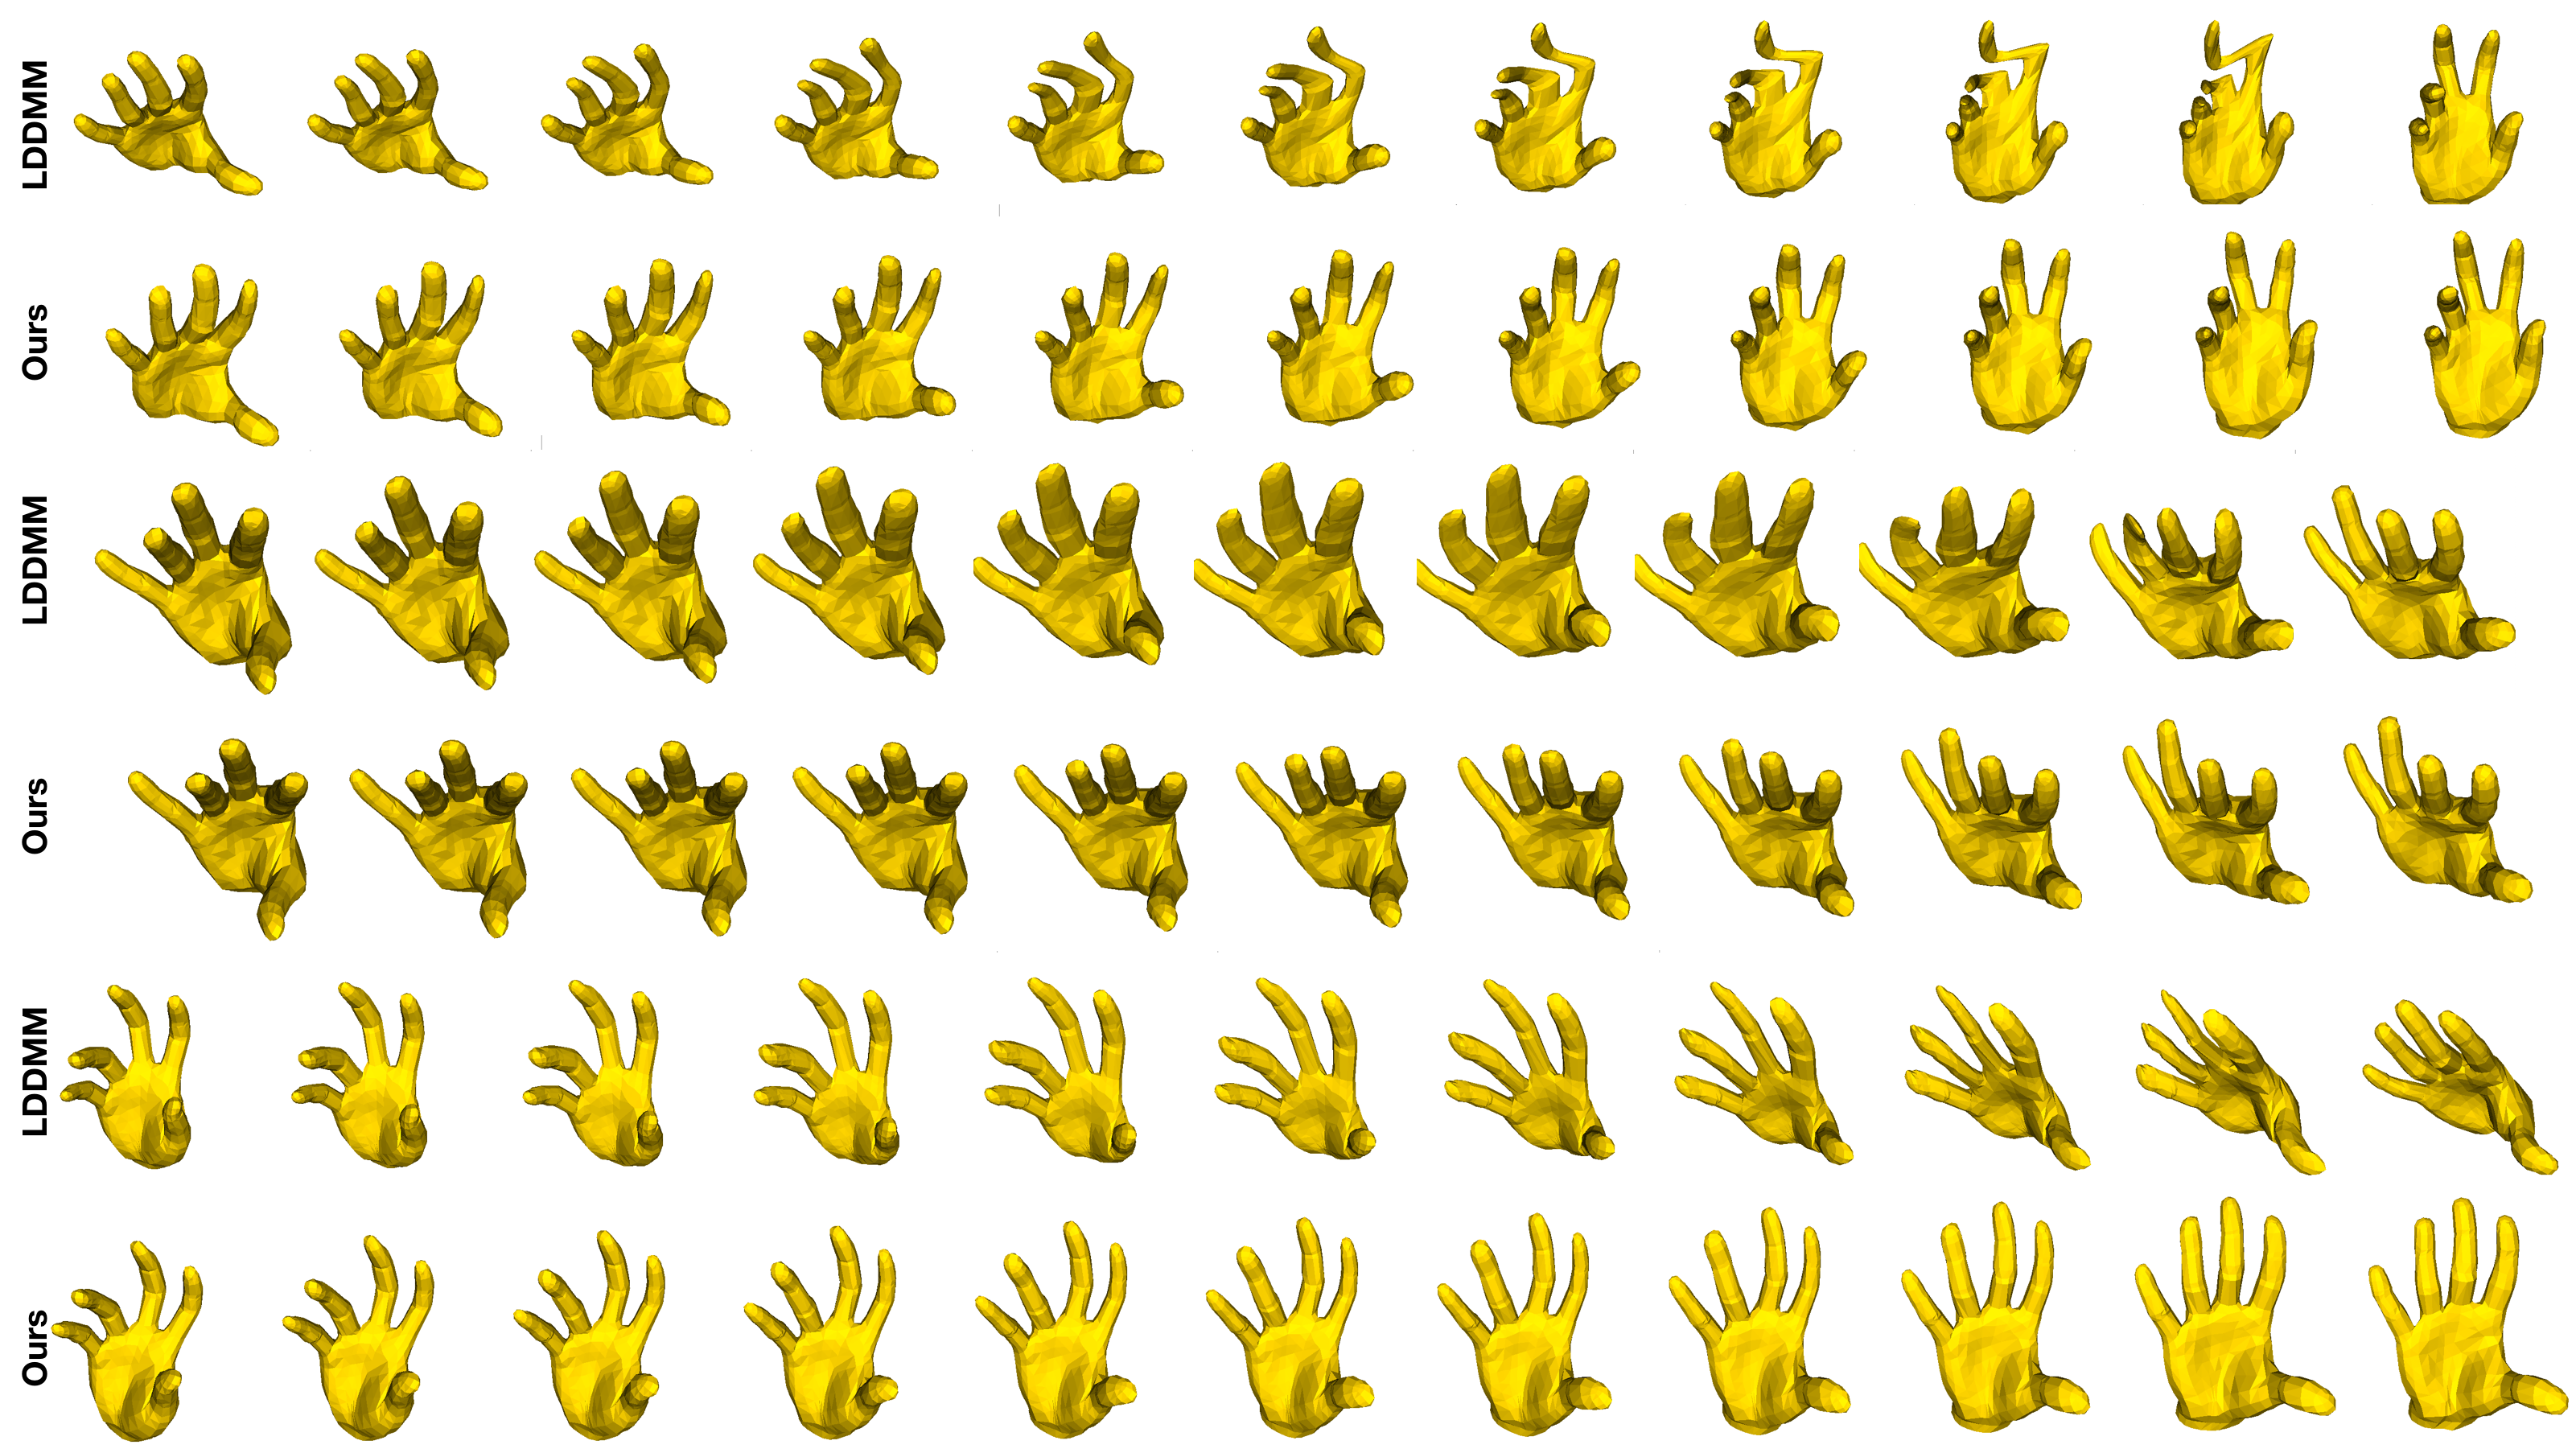
\includegraphics[width=1\linewidth]{Figs/ResNetvsLDMM.png}
%    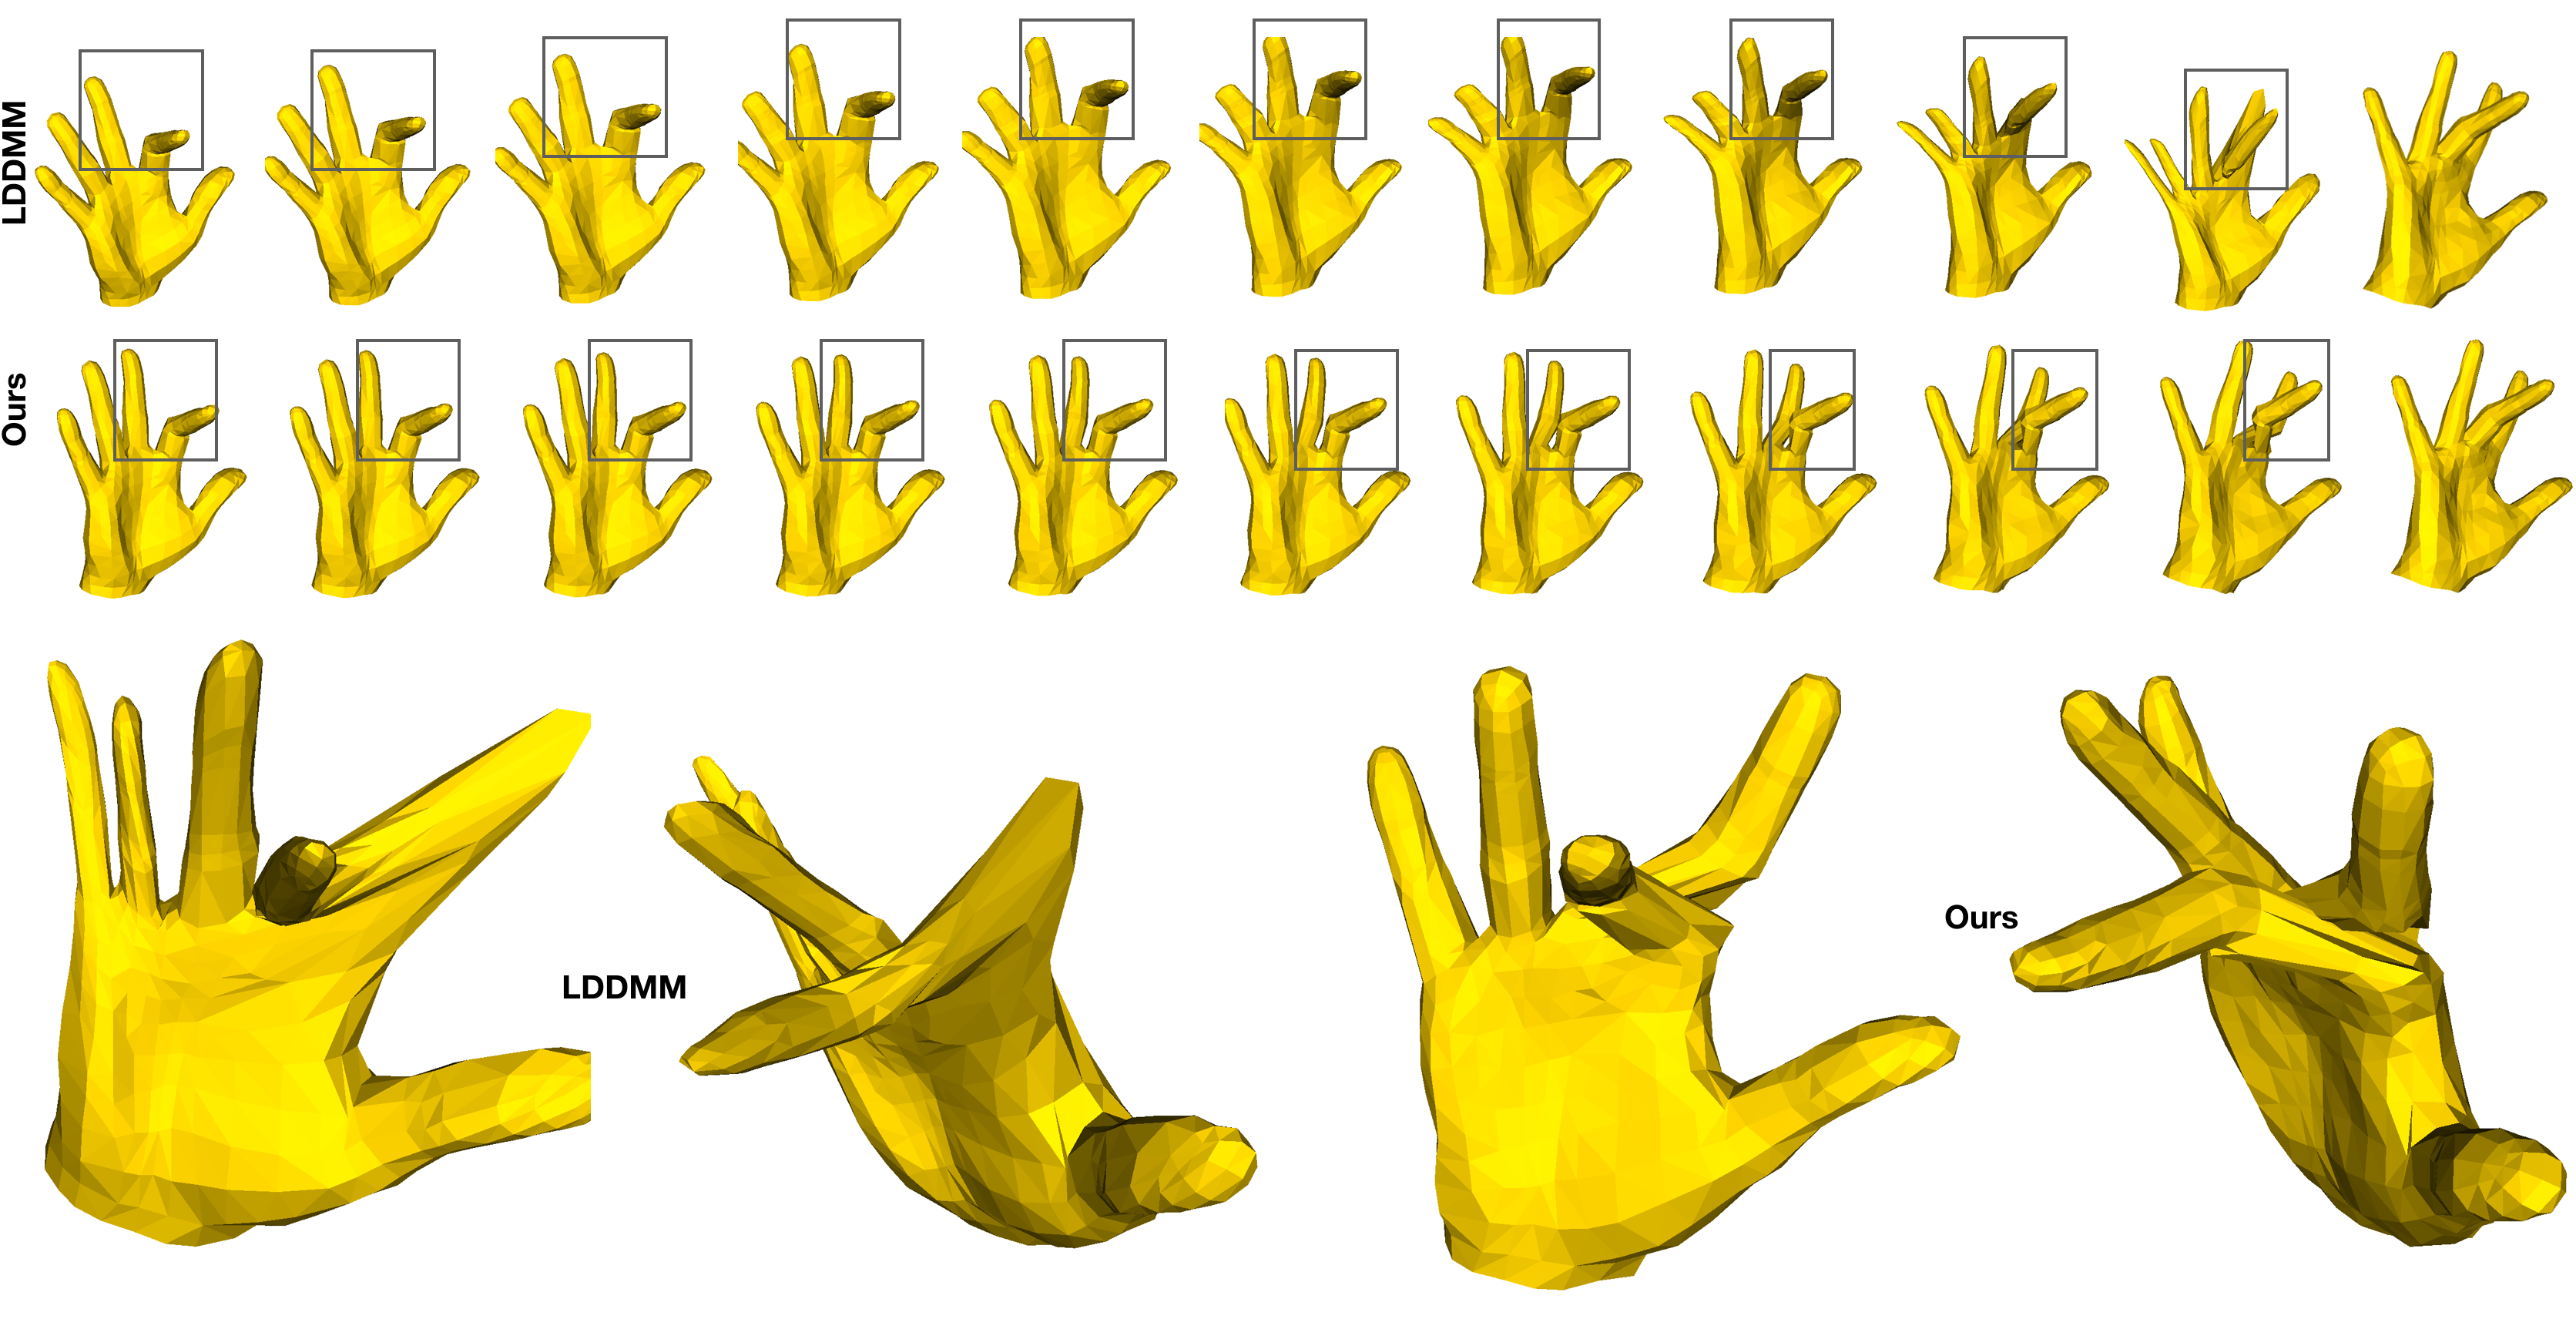
\includegraphics[width=\linewidth]{Figs/ResNetvsLDDMM-2.png}
%  \caption{Four examples to compare ResNet-LDDMM (given first) to LDDMM (given second). The last row shows obtained deformed source by LDDMM (left) and ResNet-LDDMM (right).}
%   \label{Fig:ComparisonToLDDMM}
%\end{figure}

%\begin{table*}
%\begin{center}
%\caption{Key differences between LDDMM and ResNet-LDDMM.}
%\vspace{-1}
%\begin{tabular}{c|c|c} 
%\textbf{Algorithm}  & \textbf{LDDMM} (Large Deformation Diffeomorphic Metric Mapping) & \textbf{ResNet-LDDMM} (or LDDMM Revisited) \\ 

% Problem & \multicolumn{2}{c}{Solve the \textbf{Flow Equation} (ODE) ${\partial_t \phi}(t,.) = v(t,\phi(t,.))$ s.t. at $t=0$ $\phi(0,.) = q_S$ and $\phi(1,.)$ \textbf{Diffeomorphism}.} \\
%\hline
% Paradigm & Optimize-then-Discretize (Hamiltonian formulation) & Discretize-then-Optimize (Euler discretization) \\ 
% Kernel & $K$ a predefined Gaussian kernel with a fixed scale $\sigma$ & Inferred from the data points ($K$_{NTK} when $w\to \infty$) \\
% Admissible Space & $(\cal A, \|.\|_{\cal A})$: RKHS induced by the Gaussian kernel  & $({\cal H}, \|.\|_{\cal H})$: functional space of NN $f^l(.,\theta^l)$   \\
% Kinetic Energy  & ${\cal S}(v)=\frac{1}{2} \int_{0}^{1} \langle {\cal A}v, v \rangle_{\cal A} dt=\frac{1}{2} \int_{0}^{1} \|v\|^2_{\cal A} dt$ & ${\cal S}(f)=\frac{1}{2} \int_{0}^{1}  \| f^t(.,\theta^{t}) \|_{\ell^2}^2 dt$  \\
%Regularization & Induced by the Gaussian Kernel  & Induced by the NN structure (and related NTK) \\
%Optimization & \textbf{PMP}: Pontryagin's Maximum Principle then GD  & \textbf{BP}: Backpropagation with ADAM \\
%Velocity vectors & Gaussian velocity vector fields  & Piece-wise affine in polytopes (ReLU) \\
%Computational cost & Large computational time (hours)  & Efficient computational time (minutes) \\
%\end{tabular}
%\end{center}
%\label{tab:LDDMMvsResNetLDDMM}
%\end{table*}

%To save space and make the comparison easier, we establish in Tab.\ref{tab:LDDMMvsResNetLDDMM} the key differences between LDDMM and ResNet-LDDMM. One key difference is that LDDMM are notoriously time-consuming algorithms, and while matching two shapes takes a usually acceptable amount of time, matching hundreds (or even thousands) for adequate statistical analysis can quickly become impossible. A lot of advances have being made using GPU and the free library KeOps\footnote{\url{www.kernel-operations.io}} on this front \cite{charlier2020kernel}, but it is still time-consuming to perform such analysis, especially when one needs several retries to find the correct scales for the reproducing kernel. On the other hand, ResNet-LDDMM is much faster and flexible.

%\subsubsection*{Space of Vector Fields induced by $f^l(.,\theta^l)$}

%Let's consider an arbitrary building block $l$ of our ResNet-LDDMM, it predicts a time-dependant velocity field $v^l \in \real^3$, parametrized by the subset of parameters $\theta^l$. That is, for each $x^{l-1} \in \Phi^l.q_0$, output of the previous building block, $v^l(x^{l-1})=f^l(x^{l-1},\theta^l)$. Now, consider a second point $y^{l-1}$, then we have
%$$
%\| f^l(x^l) - f^l(y^l)\|_2 \leq \|f^l\|_{\cal{A}}\|x^l - y^l\|_2
%$$

%For an arbitrary vertex $x\in q_0$, a sequence of time-dependant velocity vectors are produced according to Eq\ref{Eq:VelocityFields}  

%\begin{equation} \label{Eq:VelocityFields}
%\begin{split}
%v^l & = f^l(\Phi^{l-1}(x),\theta^l) \\
% & = W_3(W_2(\sigma(W_1\Phi^{l-1}(x)+b_1)+b_2))
% \\
% & = W_3(\tilde{v}^l)
%\end{split}
%\end{equation}

%$\theta^l = \{W_k,b_k\}_{k=1}^K$ are the ResNet parameters at the time step (or building block) $l$  and $\sigma_k$ is a Leaky ReLU activation function.

%Our time-dependant prediction functions $f^0,\dots,f^{L-1}$ are elements of a functional space $\cal A$. Non-linear operations in $\real^3$ become inner products in $\cal A$

%\begin{equation} \label{eq1}
%\begin{split}
%v^l & = f^l(\Phi^{l-1}(x),\theta^l) \\
% & = \langle f^l,\Psi(\Phi^{l-1}(x))\rangle_{\cal{A}}
%\end{split}
%\end{equation}

%The norm $\| .\|_{\cal{A}}$ is a natural regularization function:



%variations of a function $f$ in $\cal{A}$ is controlled ac- cording to this geometry...

%\subsubsection*{Relationship with NTK (Neural Tangent Kernel)}

%over-parameterized networks (that is, with large or infinite width), when considering their Gaussian process behavior.

%with sufficient over-parameterization, the (non-linear) features $x \to  \nabla_{\Theta} f(x;\theta_0)$ of the linearized model (4.1) become expressive enough to be able to perfectly fit the training data, by approximating a kernel method.

%Such over-parameterized networks are easy to optimize with gradient descent, and may converge in the infinite-width limit to a minimum-norm solution in the RKHS corresponding to a different kernel known as neural tangent kernel (NTK). 

%This kernel is given by the infinite-width limit corresponding to a feature map given by the gradient of the model with respect to its parameters, at initialization.

%\textbf{NTK for two-layer ReLU networks}

%$$
%K_{NTK} = 
%$$

%A sequence of two-layer ReLu networks with an identity map (ResNet). 

%\begin{figure}[h]
%  \centering
%   \includegraphics[width=\linewidth]{Figs/Venus.png}
%  \caption{En example of diffeomorphic registration using our ResNet-LDDMM - from left to right, source and target before registration, resulting velocity fields, models after registration, optimal path (with intermediate shapes) and absolute spatial deviation between $q^1$ and $q_T$}.
%   \label{Fig:Venus}
%\end{figure}



%\begin{figure*}[ht!]
%  \centering
%   \includegraphics[width=\linewidth]{Figs/Lena.png}
%  \caption{Smoothness of velocity vector fields -- Optimal path connecting star shapes (Lena texture mapped on the source) for a better track of the deformations.}
%   \label{Fig:GroupAction}
%\end{figure*}

%\newpage

